\documentclass[11pt]{article}
\usepackage{graphicx}
\usepackage{amsmath,amssymb}
\usepackage{amsfonts}
\usepackage{url}
\usepackage[hidelinks]{hyperref}
\begin{document}
\section*{Introduction}

\par Macroscopic freeway traffic models are widely used by transportation engineers in order to design controllers and perform re-routing or road management to improve performance of the system; for instance, increasing total traveled distance and decreasing total travel time of vehicles in the network. A crucial component of this process of traffic management is simulation of traffic behavior which is usually accomplished using traditional simulators where system's behavior is predicted by the dynamics assumed to govern evolution of traffic.

The burdensome aspect of traffic prediction is that traffic condition is contingent on too many different parameters. For instance, for a given network, the day for which the simulation is required, plays a significant role as traffic regime on weekends varies from the one on workdays. Furthermore, for a particular day, clearly, vehicular traffic in evening differs from the one at midnight. Thus, a decent traffic prediction must incorporate distinct parameters influencing traffic conditions.

\section*{Motivation}

As every watchful motorist driving in California freeways can recognize, there are numerous implemented loop detectors in freeway stretches of California that measure and record traffic metrics. These sensors provide traffic data-centers with huge amount of information that must be taken into account while making predictions. The immense existing data and complexity of traffic behavior as a result of being affected by different continuous and discrete parameters, motivated the authors to perform traffic prediction deploying neural network and deep learning methods to come up with a traffic simulation which can possibly perform better than the existing traffic simulators. 

\section*{PeMS Data} 
PeMS (Performance Measurement System) is a traffic metrics measurement system all over California deployed to obtain loop detector data in real time \cite{PemsPravin}. Freeway PeMS data consists of measurements of vehicular flow, occupancy (fraction of time a vehicle is present on the loop) and speed in time intervals of $5$ minutes. PeMS data is available to users at \url{http://pems.dot.ca.gov/}. In this project, I-210 east (Figure \ref{fig:210}) PeMS data was used as the training and validation data set. 
\begin{figure}[p]
    \centering
    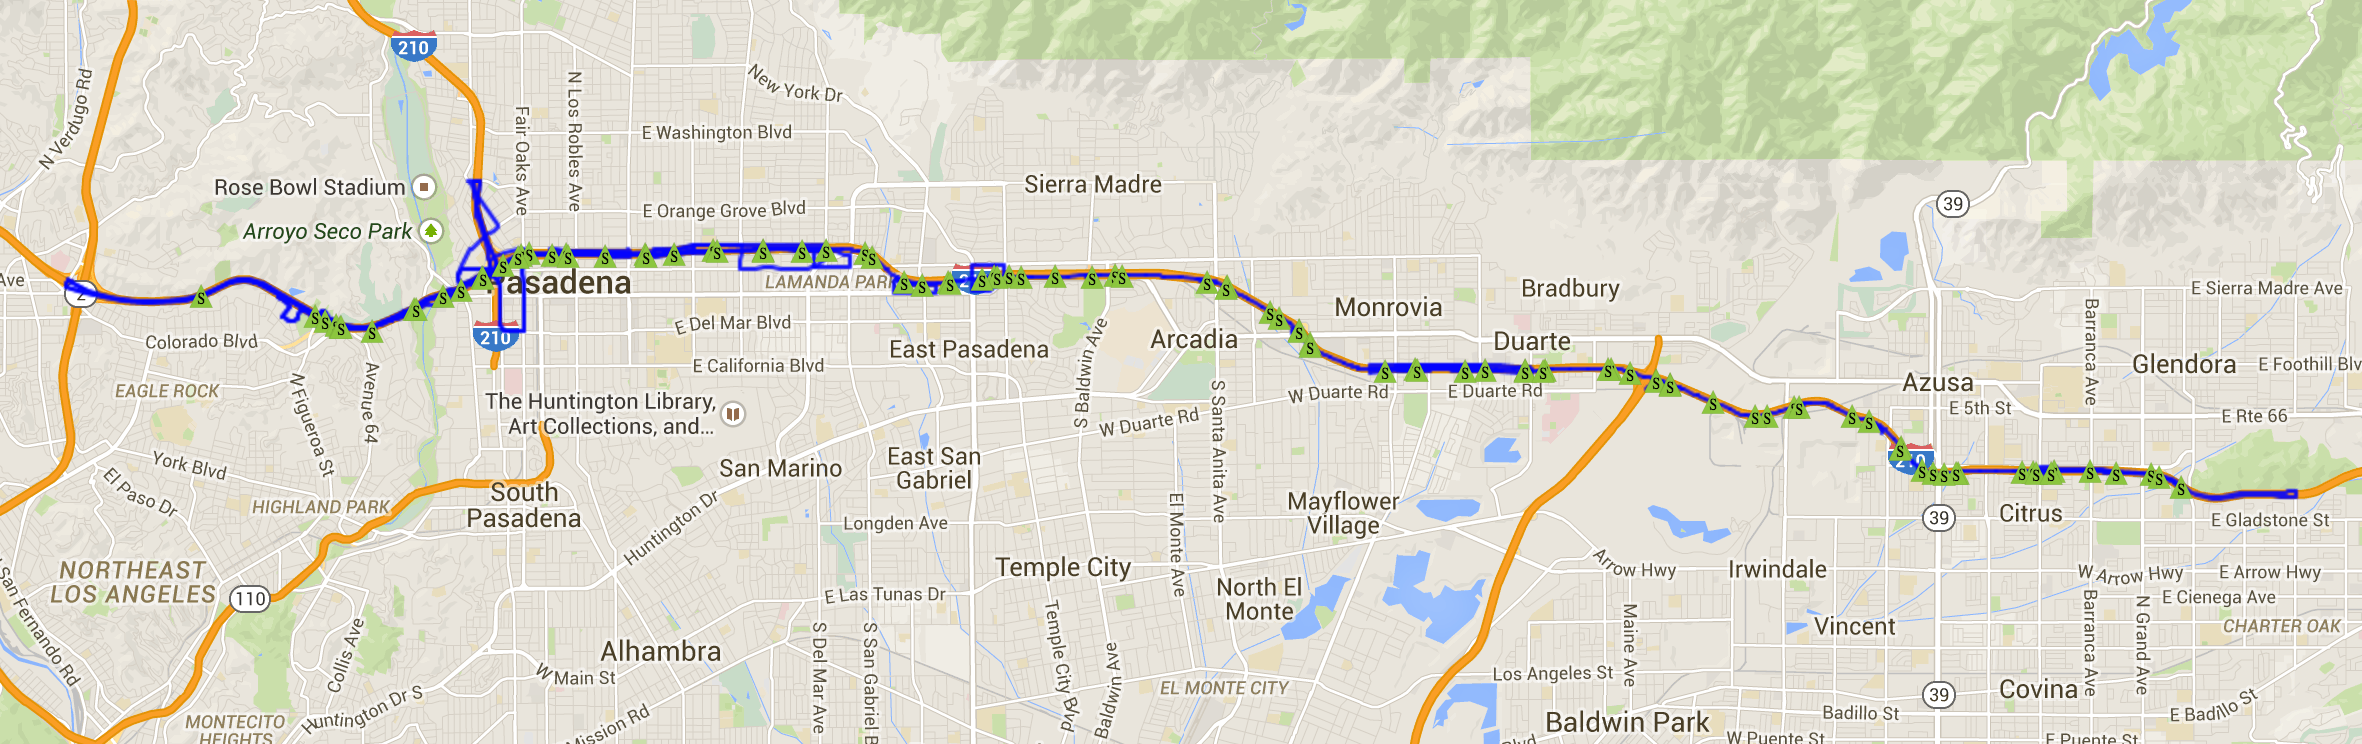
\includegraphics[width=0.8\textwidth]{210.png}
    \caption{I-210 East Topology}
    \label{fig:210}
\end{figure}  



\bibliographystyle{plain}
\bibliography{references}


\end{document}

